\subsection{Descripción del problema.}



%\vspace*{0.3cm}

%\textbf{completar!}
%\begin{figure}[htb]
%  \begin{center}
%      \includegraphics[scale=0.25]{imagenes/ejemplo.jpg}
%  \end{center}
%  \caption{ejemplo}
%\end{figure}

El objetivo de este algoritmo es obtener una configuración para una ronda de niñas exploradoras óptima, en el sentido de que la suma de las distancias entre los pares de amigas sea mínima. Cada niña es representada por una letra distinta. Se tiene como entrada del algoritmo a desarrollar para este problema una serie de niñas con algunas de sus respectivas amigas. El algoritmo debe obtener estos valores desde una archivo de texto con un formato como se puede ver en el siguiente ejemplo:


\begin{verbatim}
a bcde;b acde;c abde;d abc;e abc
a bcd;b ae;c ad;d ac;e b
a fb;b gc;d gc;f agh;e hd
x yz
\end{verbatim}

En cada linea tenemos una instancia distinta. A partir de la misma podemos obtener la cantidad total de exploradoras, y para cada una cuales son sus todas amigas. Hay que aclarar que cuando una niña es amiga de otra, esta ultima también es amiga de la primera. En la entrada solo tenemos para algunas exploradoras cuales son algunas de sus amigas. Cada string separado por un ';' indica las amistades, por ejemplo ''a bcde;'' significa que 'a' es amiga de 'b','c','d','e'. Para tener la totalidad de las amistades, se deben considerar las amistades reciprocas de las dadas originalmente, es decir también considerar que 'b', 'c', 'd' y 'e' son amigas de 'a'. Para una linea(instancia), no hay repetidos para los primeros carácteres de los string separado por un ';'. Por ejemplo para ''a dbe;b acde;c abde;d abc;e abc'',los primeros carácteres son 'a', 'b', 'c', 'd', 'e', y no se repiten. Tampoco se repiten las amistades, es decir que por ejemplo no es valida una entrada que tenga ''a dbed;'', o una misma exploradora tenga amistad consigo misma, por ejemplo ''a abed;''

Se tendrá una salida como se puede ver a continuación:

\begin{verbatim}
2 abdce
2 abecd
3 abcfgdhe
1 xyz
\end{verbatim}

Donde cada linea es la salida de una instancia, el numero representa la distancia máxima entre dos amistades dentro de la ronda. Esta última es representada por el string que sigue al número. Se considera que el primer y ultimo carácter estan unidos en la ronda.

\subsection{Desarrollo de la idea y pseudocódigo.}

%\vspace*{0.3cm}

%\textbf{completar!}

%\begin{codebox}
%\Procname{$\proc{ejemplo_de_pseudocodigo}(x,y)$}
%\li \Return $\id{solucion}$
%\end{codebox}

Para obtener la suma mínima de la distancia entre las amistades, se puede no considerar la reciproca de cada amistad. Por ejemplo si tenemos que ''a'' es amiga de ''b'', lo cual implica que ''b'' es amiga de ''a'', se puede solo considerar la distancia entre ''a'' y ''b'', pero no la reciproca.

El algoritmo del problema consiste en para cada linea del archivo de entrada, obtener un string, separarlo cada '';''. Cada elemento del arreglo contiene un string con información sobre las amistades. A partir del arreglo, construimos una lista enlazada de tuplas $ < $carácter, conjunto$ < $carácter$ > > $, donde cada elemento del conjunto es un carácter que tiene una amistad con el de la primera coordenada de la tupla. Esta lista enlazada se llama $ amistades $ en el algoritmo implementado. Para que no halla amistades repetidas, en el proceso de construir esta lista, antes de guardar un carácter en el conjunto, nos fijamos si ya había en la lista enlazada una amistad entre el elemento a agregar y la primera coordenada, en ese caso no agregamos.

Además creamos un un conjunto con los caracteres distintos que van apareciendo, para esto aprovechamos el Set de la biblioteca de java. Para utilizar la tupla se utilizara una clase especialmente creada, llamada Pair, que implementa las funcionalidades básicas de la misma. 

Luego llamamos a una función $minimaSuma$, que utilizando la lista con las amistades sin duplicados, un arreglo de char con los elementos del conjunto de exploradoras, y un arreglo de char pasado por parámetro donde se ira almacenando la palabra(representa una ronda) de suma mínima. Esta a su vez llama a la función $ minimaSumaAux $ la cual es una función que recursivamente ira calculando la suma entre las distancias de las amistades para cada permutación, para lo cual utiliza una función específica $ calcularSumaDistancias $. Para ir almacenando la suma mínima a medida que se recorren las permutaciones, se utiliza una instancia de una clase creada por nosotros llamada Entero. La misma contiene un solo campo de tipo int, y funciones get y set para manipularla. Como es un objeto, se pasa por referencia, y trabaja como un puntero que almacena un valor.
En caso de obtener una permutación con igual suma de distancias que la mínima actual, se preguntará si el es menor alfabéticamente, y en ese caso se almacenara.

Para calcular la distancia entre dos exploradoras, se toma la mínima distancia, entre las dos posibles direcciones. Para esto se calcula la distancia en un sentido, y para saber la distancia en el otro sentido se resta a la cantidad de exploradoras el anteriormente obtenido.

A continuación podemos ver los pseudocódigos de las funciones $minimaSuma$ y $ minimaSumaAux $.

\begin{codebox}
\Procname{$\proc{minimaSuma}(char[]\  original, list<caracter, Set<caracter>> \ amistades), char[]\  palabraMinima) $}
	\li \textbf{int} tam $ \leftarrow $ original.longitud
	\li \textbf{char[]} primero= new char[tam];
	\li primero[0]= original[0];
	\li \textbf{Entero} sumaMinima= new Entero(Integer.MAX_VALUE);	
	\li //lamamos a la funcion minimaSumaAux con un nivel de cero
	\li $minimaSumaAux(original, primero,0,tam,sumaMinima,palabraMinima, amistades);$
\end{codebox}

 La siguiente es la aridad de la función  $ minimaSumaAux :$ 
 
\begin{verbatim}
minimaSumaAux(char[] original, char[] agregado, int  nivel,int tam,
 Entero sumaMinima, char[] palabraMinima, List<Pair<Character, Set<Character> > > amistades)
\end{verbatim}
 
En la misma $original $ es un arreglo de char con los caracteres originales con los que se deben formar todas las permutaciones posibles. El método para efectuar esto llevado a cabo por $minimaSumaAux$ consiste en cada ''nivel'', es decir cuando la variable nivel tiene cierto valor, agregar un nuevo carácter de original a $ agregado $, y hacer todas las permutaciones posibles entre este nuevo carácter creando un nuevo arreglo de char para cada una de ellas. Por ejemplo si tenemos 

\begin{verbatim}
original=abcdef	         	agregado= cef		        nivel=3
\end{verbatim}

Hay que aclarar que $ agregado $ tiene el tamaño de la cantidad total de exploradoras, aunque solo esta completo con caracteres hasta índice nivel. Le agregamos a $agregado$ la letra indicada por nivel , en este caso la ''d'', de la siguiente manera agregado[nivel]= ''d''. Hacemos todas las permutaciones entre esta ultima y las anteriores letras de $agregado$, obteniendo.

\begin{verbatim}
cefd cedf cdfe defc
\end{verbatim}

Creamos un arreglo de char para cada una , aunque del tamaño de la cantidad de exploradoras.

Luego para cada permutación, y para el agregado modificado, llamamos recursivamente a $minimaSumaAux$, con los mismos parámetros, pero con el nivel aumentado en una unidad, y en lugar de agregado los nuevos arreglos de char. Este método nos permite crear un único arreglo de char por cada permutación.

Se ejecuta recursivamente el algoritmo hasta que llega al caso base que es cuando el nivel es el tamaño de las exploradoras, en ese caso se llama a la función $ calcularSumaDistancias $ que calcula la suma entre las distancias entre las amistades, y en caso de que la permutación en cuestión tenga menor suma, o igual, pero alfabéticamente menor, se almacenan estos valores en los objetos sumaMinima(Entero) y palabraMinima(arreglo de char).

Finalmente se llama a la función $calcularMaxDist$, que calcula todas las distancias, entre todas las amistades, y va almacenando el valor máximo.

\newpage

\subsection{Análisis de complejidad.}

%\vspace*{0.3cm}

%\textbf{completar!}

Se calcularan las complejidades en base los parámetros de entrada cantidad de exploradoras, denotado por $ n $ , y cantidad de amistades, denotado por $ a $.

En el siguiente fragmento se analiza la complejidad para una instancia, antes de llamar a $minimaSuma$

\begin{lstlisting}
String[] amistadesPuntoComa= line.split(";"); 
//es una funcion de la libreria	de java, no se encontro la documentacion con su complejidad, pero se puede estimar en a lo sumo el tamanio del string al cuadrado, con lo que seguro es menor a O( (na)^2 ).
String relacion;
List<Pair<Character, Set<Character>>> amistades= new LinkedList<Pair<Character, Set<Character>>>();
				
//contiene a las exploradoras
Set<Character> exploradoras= new LinkedHashSet<Character>()
				
for(int i=0;i<amistadesPuntoComa.length;i++){// tiene como mucho n iteraciones
	relacion=amistadesPuntoComa[i]
	char nuevoCaracter = relacion.charAt(0)
	exploradoras.add(nuevoCaracter)
	// al agregar algo a un conjunto, tiene un costo del tamanio del mismo, asi q es menor o igual a O(n)
					
//en este par guardamos todos los caracteres que se relacionan con nuevoCaracter
	Pair<Character,Set<Character> > nuevoPar =new Pair<>(nuevoCaracter,new HashSet<Character>())
	amistades.add(nuevoPar)
//empezamos desde indice dos para evitar el espacio
	for(int j=2;j<relacion.length();j++){
						
		char caracter_relacion= relacion.charAt(j)
		exploradoras.add(caracter_relacion) // nueva mente al agregar algo a un conjunto, tiene un costo del tamanio del mismo, asi q es menor a O(n)
								
		boolean hayQueGuardar=true
		for(Pair<Character,Set<Character> >  par: amistades){// seguro tiene menos o igual a n iteraciones		
			if(par.getFirst()==caracter_relacion){
				Set<Character> relaciones_caracter= par.getSecond()						
				for(Character c:relaciones_caracter){// seguro tiene menos o igual a n iteraciones							
					if(c==nuevoCaracter){
						hayQueGuardar=false
						break
						}
				}				
				break
			}					
		}// tenemos un costo de menor o igual a O(n^2) este ciclo
		if(hayQueGuardar){
			nuevoPar.getSecond().add(caracter_relacion) //puede tener un costo como mucho de O(n) ya que agregamos algo a un conjunto
		}
	}
} al finalizar este ciclo tenemos un costo menor o igual a O(n^3*a^2)

//con un iterador pasamos el Set de exploradoras a un arreglo de char, con un costo de O(n)
char[] original= new char[exploradoras.size()]
Iterator<Character> itExpl= exploradoras.iterator()
int indice=0
while(itExpl.hasNext()){
	original[indice]=itExpl.next()					
	indice++
}
					
int tam= original.length
char[] palabraMinima= new char[tam]	
minimaSuma(original,amistades,palabraMinima)
\end{lstlisting}

Se tiene un costo menor o igual a $ O(n^{3}a^{2}) $ antes de llamar a $ minimaSuma $ por lo que el orden de la complejidad estará dominado por esta ultima función.

A continuación se detallan algunas de las funcione auxiliares utilizadas, con sus complejidades. 

\begin{lstlisting}

	public static int calcularDistancia(char[] instancia, int desde,char c){
		
		int dist=0
		int indice=desde
		 for(int j=0;j<instancia.length;j++){ // a lo sumo n iteraciones	 
			 dist++ 
			 indice++ 
			 indice %=instancia.length;
			 
			 if(instancia[indice]==c){
				 break
			 }	 
		 } 
		 return Math.min(dist, instancia.length-dist);
	}

\end{lstlisting}

Como la función utiliza a lo sumo n iteraciones, tiene un costo de O(n).


\begin{lstlisting}
public static int calcularSumaDistancias(char[] instancia, List<Pair<Character, Set<Character> > > amistades){
		
	int sumaDistancia=0
	int distanciaCaracter
	for(int i=0;i<instancia.length;i++){ //exactamente n iteraciones
		char c1= instancia[i]
		for(Pair<Character, Set<Character> > par: amistades){ //a lo sumo n iteraciones
			if(par.getFirst()==c1){
				for(char c: par.getSecond()){// a lo sumo n iteraciones
					distanciaCaracter= calcularDistancia(instancia,i,c) // costo a lo sumo O(n)
					sumaDistancia +=distanciaCaracter					
				}//costo de cada iteracion de este ciclo O(n)
			break	
			}				
		}
	}
	return sumaDistancia
}
\end{lstlisting}

Como el tercer for anidado del anterior fragmento solo se ejecuta para una de las n iteraciones del segundo for(debido al condicional if) los podemos considerar a los dos como uno solo con un costo igual al del tercer for sumado a un costo de $O(n)$ en peor caso. La cantidad total de veces que se ejecuta el cuerpo del tercer for es menor o igual a la cantidad de relaciones, y como el costo de cada un es $O(n)$, tenemos un costo total de $O(na)$. Como se mensionó, para cada iteración del primer ciclo, además del costo del tercer ciclo, tenemos un costo de O(n), con lo que tenemos un costo adicional de $O(n^2)$. De esta forma podemos decir que el costo de esta función es $O(n^2+na)$ o $O(an^2)$



%Como esta es una función que se utilizara para cada permutación, se podría mejorar la implementación para reducir la complejidad de la misma, estableciendo previamente una relación entre cada carácter y sus amistades especificadas en la lista enlazada, de manera de poder acceder en forma directa para cada carácter a sus amistades.



El siguiente es un fragmento del código de la función $ minimaSuma$, en el mismo podemos ver que la complejidad esta dominada por $ minimaSumaAux $.
\begin{lstlisting}
	private static void minimaSuma(char[] original, List<Pair<Character, Set<Character> >  > amistades, char[] palabraMinima){
		
		int tam= original.length	
		char[] primero= new char[tam]
		primero[0]= original[0]
		Entero sumaMinima= new Entero(Integer.MAX_VALUE)
		minimaSumaAux(original, primero,0,tam,sumaMinima,palabraMinima, amistades)
}
\end{lstlisting}

En el siguiente fragmento podemos encontrar el código de la función $ minimaSumaAux $.

\begin{lstlisting}

	private static void minimaSumaAux(char[] original, char[] agregado, int nivel,int tam, Entero sumaMinima, char[] palabraMinima, List<Pair<Character, Set<Character> >  > amistades){
		
		if(nivel==tam-1){// caso base
						
			int sumaDistancia= calcularSumaDistancias(agregado, amistades);//O(a*n^2)
			if(sumaDistancia<sumaMinima.getValor()){// este if en peor caso O(n)
				
				sumaMinima.setValor(sumaDistancia)	
				for(int j=0;j<tam;j++){//O(n)
					palabraMinima[j]=agregado[j]
				}//costo de O(n)		
			}	
			if(sumaDistancia==sumaMinima.getValor() && esMenor(agregado,palabraMinima)){// tambien este if en peor caso O(n)
				
				//guardamos la palabra minima
				for(int j=0;j<tam;j++){
					palabraMinima[j]=agregado[j]
				}
			}
			return; // tenemos un costo de caso base de O(a*n^2) en peor caso
		}
		
		
		int nuevoNivel=nivel+1
		char nuevoCaracter =original[nuevoNivel]

		List<char[]> permut = new LinkedList<char[]>()
		agregado[nuevoNivel]=nuevoCaracter
		permut.add(agregado)
		for(int i=0;i<=nuevoNivel-1;i++){
			
			char[] aAgregar = new char[tam]// a lo sumo alojar un arreglo en memoria, un costo de O(n)
			for(int j=0;j<=nuevoNivel;j++){	
				aAgregar[j]=agregado[j]		
			}//costo de O(nuevoNivel)
			
			swap(aAgregar,i,nuevoNivel)	//costo O(1)
			permut.add(aAgregar)
			
		}//costo de O(nivel*n) antes de llamar recursivamente

		for(char[] arr: permut){
			//se llama recursivamente a la misma funcion, pero esta esta mas cerca del caso base
			minimaSumaAux(original, arr,nuevoNivel, tam, sumaMinima, palabraMinima, amistades);		
		}
		
		permut.clear()
		
	}
\end{lstlisting}


Para calcular la complejidad, si en lugar de hacerlo con una ecuación de recurrencia, se tiene en cuenta que el caso base se ejecuta para cada una de las permutaciones posibles, que el costo de crear y ordenar cada arreglo de char es $ O(n) $, y que hay exactamente uno por permutación, como hay$ n! $ permutaciones, tenemos un costo de $ O(n!(n+an^2)$, lo que es equivalente a $ O(an!n^2)$. 

Para obtener la complejidad $ T_1(n) $ de la función $ minimaSumaAux $, podemos plantear una función $ T(nivel,n) $ que calcula la cantidad de operaciones elementales por nivel que realiza la anterior función, en el sentido de que para el nivel n se consideran todas las operaciones de nivel superior. Decimos que una operación elemental esta en un cierto nivel si es llamada desde una función $ minimaSumaAux $ con ese parámetro en el campo nivel. De esta manera para obtener la complejidad $ T_1(n) $, evaluamos $T(0,n)$. Pero para esta nueva función, podemos plantear una ecuación de recurrencia.

\begin{equation*}
T(nivel,n) = \left\lbrace
\begin{array}{c}
 (nivel+2)T(nivel+1)+(nivel+1)n) \ \ \ si \ \ \ \  nivel< n-1 \\
  an^2  \  \ \ \  \ si \ \ \ \  nivel==n-1 \\
\end{array}
\right.
\end{equation*}

Para obtener  $T(0,n)$, podemos expandir la evaluación:
\begin{equation*}
\begin{array}{c}
 T(0,n)=2T(1,n)+n=2(3T(2,n)+2n)+n=3!T(2,n)+2^{2}n+n= \\
  = 3!(4T(3,n)+3n)+2^{2}n+n=4!T(3,n)+3^{2}2!n+2^{2}1!n+n=\cdots\\
 \cdots = n!(n^2a) + \sum_{i=0}^{n-1} (i+1)^{2}i! n  \\
\end{array}
\end{equation*}

Seguro podemos acotar a la función de complejidad resultante por una de la forma $ n!p(n)a $, con p un polinomio, por lo que su complejidad seguro pertenece a $O(n!p(n)a)$.

Como antes de llamar a la función $ minimaSuma $ se tenía un costo de $ O(n^{3}a^{2})$, tenemos un costo total para el algoritmo del ejercicio 3 que pertenece a $ O(n!p(n)a^2)$.

El orden de la complejidad es estrictamente menor que $ O(a^2n^n)$, ya que vale que $ O(n!p(n)) $ con p un polinomio, es estrictamente menor que $ O(n^n) $.

Finalmente se llama a a función $calcularMaxDist$, para calcular la máxima distancia entre pares de amigas. Su costo computacional se calcula igual que para la función $calcularSumaDistancias$, y es el mismo.

 Como para todas las instancias de entrada se hacen todas las permutaciones y para cada una se calcula la suma para ver si es menor a la suma acumulada, no hay grandes diferencias entre peor caso y mejor caso.
 
 
 



\subsection{Correctitud}

Para garantizar que nuestro algoritmo es solución del problema, se tiene que cumplir que se evalue $ calcularSumaDistancias $ para todas las permutaciones posibles. Para esto se tiene que cumplir que la forma en que las construimos abarca todos los casos. En el siguiente ejemplo, podemos ver que para cada nivel de la función $minimaSumaAux$, se obtienen todas las permutaciones posibles


\begin{figure}[H]
\centering
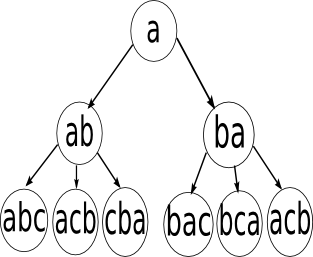
\includegraphics[scale=0.8]{imagenes/ej3Correctitud.png}
\caption{Permutaciones posibles para }
\label{256value}
\end{figure}



Podemos describir que lineas generales el método, el cual se explico en la sección anterior, consiste en tomar en cada paso, todas las permutaciones generadas en el paso anterior, agregarle un nuevo caracter a todas, y construir todas las secuencias resultantes de intercambiar el nuevo caracter con los demás caracteres, incluyendo la que solo le agrega al final el nuevo.

Demostraremos por inducción en la cantidad de pasos, que el método llevado a cabo por nuestro algoritmo, genera todas las permutaciones.

Para esto demostraremos dos proposiciones previas:

\begin{itemize}
\item En el paso $ n $ tenemos secuencias de $ n $ elementos.
\item En el paso $ n $ tenemos $ n! $ secuencias.
\item Las permutaciones obtenidas en cada paso son todas distintas.
\end{itemize}

Con estas tres ultimas podemos, y usando que la cantidad de permutaciones de una secuencia de $ n $ elementos es $ n! $, podemos demostrar que en cada paso se tiene la cantidad maxima de permutaciones para un dado tamaño de secuencia. Se tiene la máxima cantidad, si tiene $ n! $, y no tiene secuencias repetidas.

La primera proposición se puede probar en forma trivial por inducción en la cantidad de pasos.

Probemos también por inducción la segunda proposición. 

El caso base se cumple de manera trivial para $ n=1 $, ya que tenemos una secuencia, lo cual coincide con $1! $. 

Veamos el paso inductivo, es decir que si vale en el paso $ n $, entonces vale en el paso $ n+1 $. 

Sabemos que en el paso $ n $ hay $ n! $ secuencias(HI), veamos que en el paso $ n+1 $ hay $ (n+1)! $ secuencias. Par cada una de las secuencias de $ n $ elementos, en el paso $ n+1 $ construimos las $ n+1 $ instancias que surgen de intercambiar el nuevo carácter agregado con un solo carácter de los anteriores, incluyendo la secuencia en que no se intercambia el nuevo carácter agregado. Como se tienen $ n+1 $ secuencias, para cada una de las secuencias del paso anterior, y en este último había $ n! $, tenemos un total de $ (n+1)n! $ en el nuevo nivel, es decir $ (n+1)! $, como queríamos probar.

La tercer proposición, nuevamente se probara por inducción, pero se utilizará fuertemente el siguiente lema:
\bigskip

\textbf{Lema 1:} Si tengo un conjunto de secuencias distintas, con el último carácter igual, al generar todas las posibles secuencias que resultan de permutar el último carácter, con alguno(solo uno) de los restantes, inclulléndose, tenemos que todas las obtenidas son distintas.
\bigskip

Procedemos a demostrar el lema, utilizando el absurdo. Supongamos que entre dos secuencias distintas hacemos un intercambio entre el último carácter, y algún índice(puede ser distinto entre ambas), obteniendo dos secuencias iguales.

Separamos en casos:

\begin{itemize}
\item Si el ultimo carácter se intercambia con índices distintos,tenemos que estas nuevas secuencias difieren en el índice donde se inserto el último carácter, abs.
\end{itemize}


\begin{itemize}
\item Si el ultimo carácter se intercambia con índices iguales
	\begin{itemize}
		\item En caso de que en las palabras el elemento del índice con que se intercambia es distinto, tenemos que las nuevas secuencias difieren en el último carácter, abs 
		\item En caso de que sean iguales los caracteres(y el índice), como las secuencias originales eran distintas, debe existir algún otro índice en que difieran en un carácter. Este índice no fue modificado, así que las secuencias siguen siendo distintas.
	\end{itemize}
\end{itemize}

Ahora procedemos a probar inductivamente la tercer proposición. El caso base es trivial ya que para un paso, todas las secuencias son distintas, ya que hay una sola. Para probar el paso inductivo, utilizamos el lema anterior.
\subsection{Validación}

Se corroboro que pasen los test de la cátedra. Se verifico que se ejecute correctamente para un archivo de entrada especialmente preparado con casos borde llamado $ Ej3\_validacion.in $, y se observo que la salida era aceptable. Para cada instancia de test ejecutada, se verifico imprimiendo por pantalla que el arreglo de tuplas llamado $ amistades $ contenía los caracteres esperados. Se imprimió por pantalla la suma mínima obtenida, y se verificó que coincidía con la suma de distancias calculada a mano. Las funciones para imprimir esto en pantalla se encuentran comentadas.

Para verificar que se probaron todas las permutaciones posibles, se utilizo una lista enlazada en la cual se guardaban todas las instancias. Se verificó que la misma no tenia repetidos, y que su cantidad era n!. La misma se llamaba $ recolectadas $ y se encuentra comentada en el código, para utilizarla se debe además utilizarla de parámetro en $minimaSumaAux$, ya que que en el código entregado no se encuentra esta funcionalidad. No obstante no se puede utilizar esta lista en caso de que la cantidad de caracteres sea mayor a cierto numero, porque se gastaría mas memoria del que soporta la maquina. En este sentido se corroboro que para la ultima instancia de $ Ej3\_validacion.in $ la maquina no se queda sin memoria, verificándose que el programa no se gastan mas de 230 Mb, y no tarda mas de dos horas en ejecutarse. En caso de utilizar la lista enlazada para esta instancia, la maquina se queda sin memoria.


\newpage
\subsection{Experimentación}

En una experiencia se dejo fijo el ''a'' en 7, y se vario el ''n'' desde 8 a 13. Se corrió dos veces(para tomar promedio) el algoritmo, utilizando la clase $Ejercicio3$, con una pequeña modificación para medir tiempos e imprimirlo en pantalla, la cual fue borrada posteriormente. En la figura~\ref{aCte} podemos visualizar los resultados.

\begin{figure}[H]
  \begin{center}
      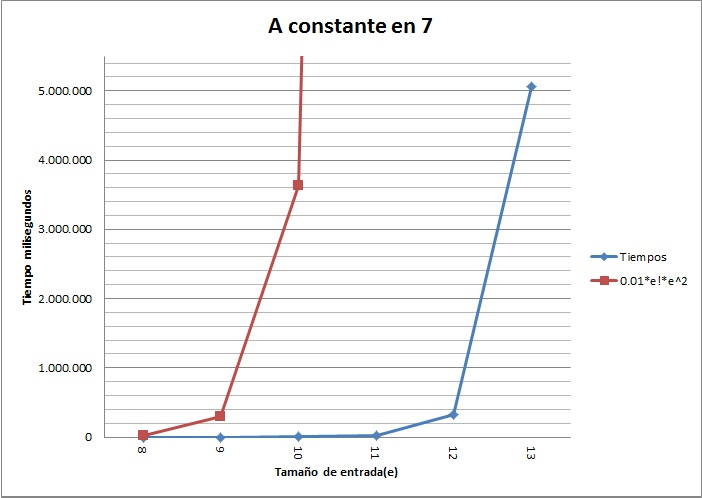
\includegraphics[scale=0.75]{imagenes/GraficoEj3Aacotado7.jpg}
  \end{center}
  \caption{En azul encontramos el gráfico de tiempos obtenidos en función de n, en rojo el gráfico de una función con un comportamiento similar}
  \label{aCte}
\end{figure}

También se constato que el tiempo para un ''n'' de 14, el tiempo era mayor a 15 hs. En base a estos resultados, esperamos que para una cantidad de exploradoras mayor, el tiempo esperado sea mucho mayor aun.

Para otra experiencia se dejo fijo el ''n'' en 12, y se vario el ''a''. Nuevamente se corrió dos veces, para tomar promedio, el algoritmo, utilizando la clase $Ejercicio3$, con una pequeña modificación para medir tiempos e imprimirlo en pantalla. En la figura~\ref{nCte} podemos ver los resultados obtenidos.

\begin{figure}[H]
  \begin{center}
      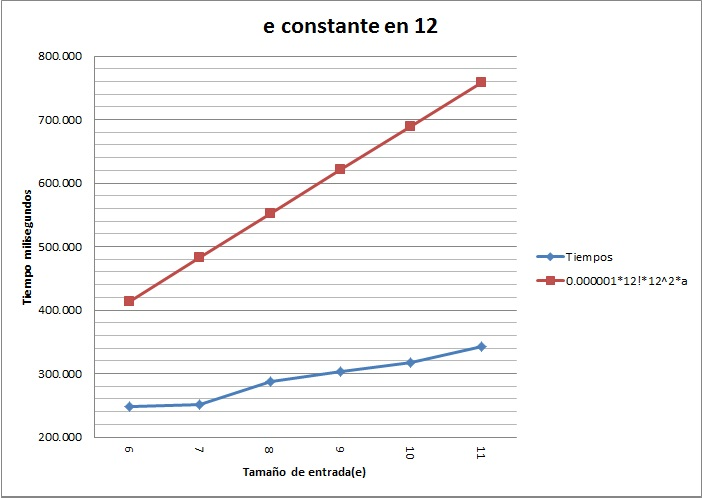
\includegraphics[scale=0.75]{imagenes/GraficoEj3Ncte12.jpg}
  \end{center}
  \caption{En azul encontramos el gráfico de tiempos obtenidos en función de n,en rojo el gráfico de una función con un comportamiento similar}
  \label{nCte}
\end{figure}

Según nuestro calculo de complejidad, al no tener la especificación de la función $ split $ de la clase $ String $ de java, no sabiamos si la complejidad final dependía de $ a $ o de $a^2$. Sin embargo como el termino $a^2$, no multiplica a $ n! $, no tiene relevancia en la complejidad final. Con los resultados obtenidos podríamos decir que es lineal, los puntos podrían ser ajustados por una función lineal de una cierta pendiente y ordenada al origen.
